\documentclass[12pt, a4paper, uplatex]{jsarticle}
\usepackage[dvipdfmx]{graphicx}
\title{アルゴリズム第2B 期末レポート}
\author{62213887 中川 和親}
\begin{document}
\maketitle

\section{概要}
本レポートでは、アルゴリズム第2Bのゲームアルゴリズムにおける
ミニマックス法とその評価関数の比較を行う。

\section{実装について}
\subsection{実装方法}
Swiftを用いる。プログラムに際してはGitHub Copilotを活用したが、あくまで補完機能の延長線上にとどめた。
Swiftの採用理由としては、絵文字の出力が画一的に対応していることなどが挙げられる。
macOSのユーザでかつXcode Command Line Toolsをインストールしている人は標準でSwiftが使えるため、
再現性においても有利であると考えた。Linuxでも使うことができ、
今回は外部ライブラリを使わないため、環境を汚すことなく実行できる。
ソースコードは全てGitHubにアップロードしている。

\subsection{実装内容}
実装の難易度の関係から、以下のルールは実装しなかった。
\begin{itemize}
  \item キャスリング
  \item アンパッサン
  \item プロモーション
  \item 50手ルール
\end{itemize}

\section{評価関数について}
2種類用意した。
\subsection{コマの価値に準じた評価関数 Offensive関数}
私が習っていた頃のチェスにおいては、表\ref*{tab:piece_value}のような価値基準が定番であった。
\begin{table}
  \centering
  \caption{コマの価値}\label{tab:piece_value}
  \begin{tabular}{|c|c|}
    \hline
    駒     & 価値       \\
    \hline
    ポーン   & 1        \\
    ナイト   & 3        \\
    ビショップ & 3        \\
    ルーク   & 5        \\
    クイーン  & 9        \\
    キング   & $\infty$ \\
    \hline
  \end{tabular}
\end{table}
キングは無限なので、今回は十分に大きい1000とする。
自サイドのコマの価値の合計から相手サイドのコマの価値の合計を引いたものを評価値とする。
この評価関数では、相手のコマを取ることを重視することが予期されるため、
Offensive関数と名付けた。
図\ref{fig:offensive}は、評価関数の実装である。
\begin{figure}
  [h]
  \centering
  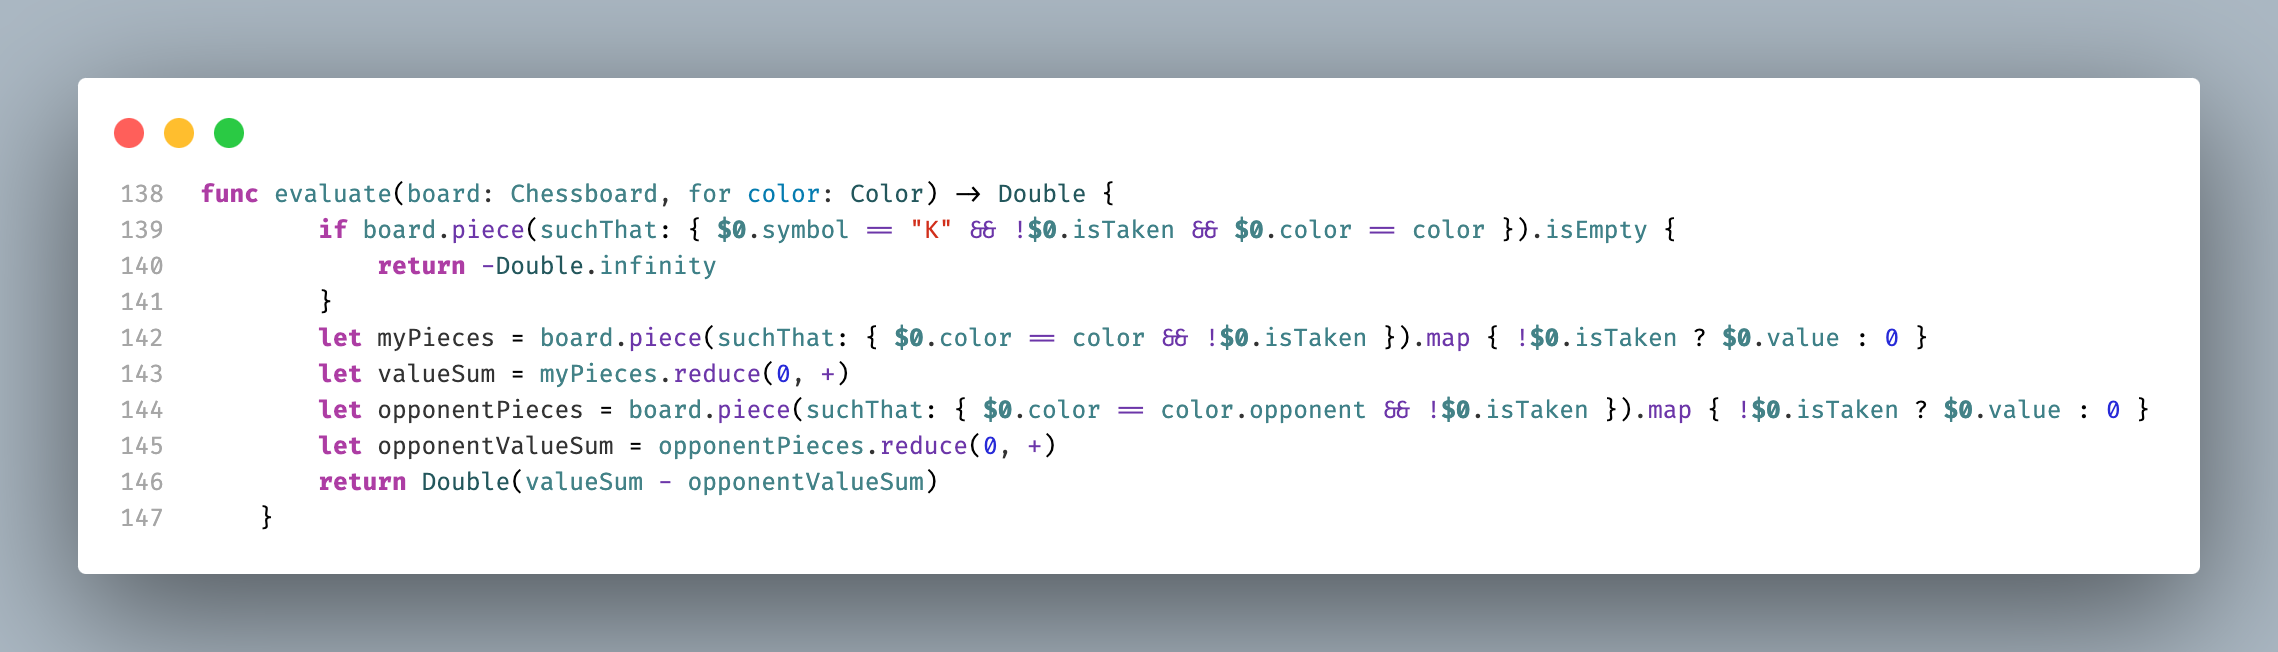
\includegraphics[width=\textwidth]{OffensiveEvaluator.png}
  \caption{Offensive関数の実装(Player.swift)}\label{fig:offensive}
\end{figure}

\subsection{手数の多さの評価関数 Strategic関数}
手数が相手より多いほど評価値が高くなるようにし、キングを取ると評価値が最高、取られると評価値が最低になるようにした。
手数が多いということは、コマが中央やひらけた位置に配置できているということであり、コマを強い状態に保てていることを意味する。
また、相手の手数を少なくすることは、相手のコマを取ることにもつながるため、優秀であると考える。
コマをより多く出陣させることから、Strategic関数と名付けた。
図\ref{fig:strategic}は、評価関数の実装である。
\begin{figure}
  [h]
  \centering
  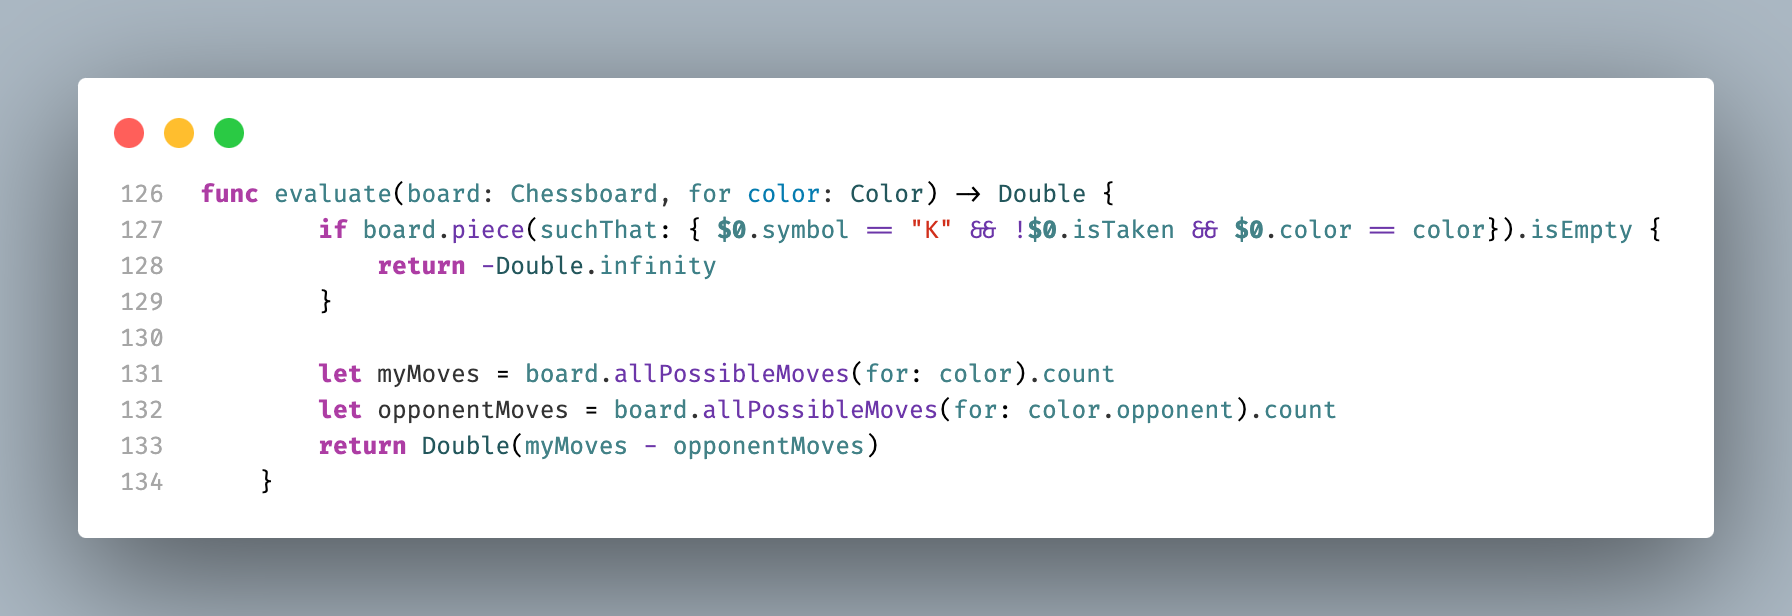
\includegraphics[width=\textwidth]{StrategicEvaluator.png}
  \caption{Strategic関数の実装(Player.swift)}\label{fig:strategic}
\end{figure}

\section{minimaxの実装部分}
図\ref{fig:minimax}は、minimax法の実装である。今回はdepthを3に設定した。
\begin{figure}
  [h]
  \centering
  \includegraphics[height=0.6\textheight]{minimax.png}
  \caption{minimax法の実装(Player.swift)}\label{fig:minimax}
\end{figure}
当初はシングルスレッドでの動作を想定していたが、時間がかかりすぎたため、
DispatchQueueなどを用いてマルチスレッドでの動作を実現した。

\newpage
\section{結果}
\subsection{勝敗}
\subsubsection{OffensivePlayer 対 RandomPlayer}
以下のコマンドを実行すると、OffensivePlayerがRandomPlayerに勝利することが確認できる。
RandomPlayerはランダムに手を選ぶプレイヤーである。
\begin{verbatim}
  swift run Chess O vs R
\end{verbatim}
乱数による結果ではあるが、OffensivePlayerが勝利することが多い。
棋譜は付録に示す。
--stepオプションをつけるとエンターキーで次の手を進めることができるので実際に試合を見たい場合に活用いただきたい。
\begin{verbatim}
  swift run Chess O vs R --step
\end{verbatim}

また、棋譜を打ち込みたい場合、
\begin{verbatim}
  swift run Chess H vs H
\end{verbatim}
上部のコマンドを実行すると互いに手を打ち合って対戦できる。
付録の試合を再現できると考えられる。

\subsubsection{StrategicPlayer 対 RandomPlayer}
以下のコマンドを実行すると、StrategicPlayerがRandomPlayerに勝利することが確認できる。
\begin{verbatim}
  swift run Chess S vs R
\end{verbatim}
棋譜は付録に示す。

なお、最後の盤面は以下の通りである。
\begin{figure}
  [h]
  \centering
  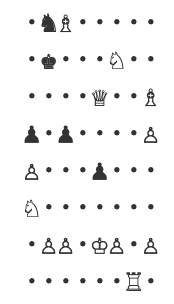
\includegraphics[width=0.5\textwidth]{LastChessboard.png}
  \caption{最終盤面}\label{fig:final}
\end{figure}
白の方が強く多いコマを持っていることがわかる。チェックメイトで終了していないのは、
ランダムに選ぶプレイヤーがキングを守る手を選ばなかったためである。

\subsection{OffensivePlayer 対 StrategicPlayer}
以下のコマンドを実行すると、OffensivePlayerがStrategicPlayerに勝利することが確認できる。
\begin{verbatim}
  swift run Chess O vs S
\end{verbatim}

結果の棋譜は付録に示した。結果は引き分けであったが、図\ref{fig:finally}の盤面からもわかるように、
OffensivePlayerが有利であることがわかる。

\begin{figure}
  [h]
  \centering
  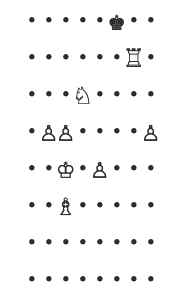
\includegraphics[width=0.5\textwidth]{Finally.png}
  \caption{最終盤面}\label{fig:finally}
\end{figure}

\section{時間的優位性}
OffensivePlayerは、StrategicPlayerに比べて思考時間が短い。
実際に計測した結果では、OffensivePlayerは約726秒、StrategicPlayerは約8476秒であった。
OffensivePlayerは相手のコマを取ることを重視しているため、
コマをとると手数の削減につながるため、思考時間が短くなると考えられる。
一方で、StrategicPlayerは手数の多さを重視しているため、思考時間が長くなると考えられる。

\section{結論}
StrategicPlayerもOffensivePlayerもRandomPlayerに勝利することができたため、
評価関数としてはどちらも有効であると考えられる。
ただ、OffensivePlayerの方が思考時間が短い上にOffensivePlayerに対し有利に試合を進めたいたため、
OffensivePlayerを採用することが望ましいと考えられる。

\section{付録}

\subsection{StrategicPlayer 対 RandomPlayer}
\begin{verbatim}
  ~~~
  Checkmate
  White : d4
  Black : g5
  White : Nc3
  Black : g4
  White : h3
  Black : b5
  White : hxg4
  Black : c5
  White : dxc5
  Black : d6
  White : Qd2
  Black : a5
  White : Qd5
  Black : Bxg4
  White : Qxa8
  Black : Bc8
  White : Qxb8
  Black : Nf6
  White : Nxb5
  Black : Rg8
  White : Qc7#
  1.0 - 0.0
  \end{verbatim}

\subsection{OffensivePlayer 対 RandomPlayer}
\begin{verbatim}
  White wins
  White : d3
  Black : b5
  White : Qa5
  Black : e6
  White : Bg5+
  Black : Ne7
  White : e4
  Black : Ba6
  White : Qc3
  Black : c6
  White : d4
  Black : d6
  White : d5
  Black : Kc8
  White : Nf3
  Black : exd5
  White : Nd4
  Black : Ng6
  White : Qe3
  Black : Qd7
  White : Nf5
  Black : Kc7
  White : g4
  Black : Nf4
  White : Qc3
  Black : Qc8
  White : Bxf4
  Black : h6
  White : Rg1
  Black : c5
  White : a4
  Black : g5
  White : Ra3
  Black : Kb7
  White : Qf6
  Black : b4
  White : Bxa6+
  Black : Kc6
  White : Bxc8
  Black : h5
  White : Ke2
  Black : dxe4
  White : Qxf7
  Black : Rh6
  White : Bxg5
  Black : bxa3
  White : Nxa3
  Black : Re6
  White : Qxe6
  Black : a5
  White : gxh5
  Black : Bh6
  White : Bxh6
  Black : Ra7
  White : Nxd6
  Black : Rf7
  White : Nxf7+
  Black : Kb6
  White : Bxb7
  1.0 - 0.0
\end{verbatim}

\subsection{OffensivePlayer 対 StrategicPlayer}
\begin{verbatim}
Stalemate
White : b3
Black : d6
White : Nc3
Black : Bg4
White : Nb1
Black : Qb5
White : Na3
Black : Qd5
White : Rb1
Black : Nc6
White : Ra1
Black : Nd4
White : h4
Black : Kd7
White : Rh2
Black : g6
White : f3
Black : Bh6
White : fxg4
Black : Nf6
White : Qg3
Black : Ne4
White : Qe1
Black : Bf4
White : Rh3
Black : Qc5
White : e3
Black : Ne2
White : Kxe2
Black : Bg3
White : Rxg3
Black : a5
White : Rh3
Black : a4
White : Kd3
Black : Qb4
White : Nb1
Black : a3
White : Rh2
Black : d5
White : Rh1
Black : h5
White : gxh5
Black : Rxh5
White : g4
Black : Rh8
White : Nh3
Black : g5
White : c3
Black : Qb6
White : Bg2
Black : f5
White : gxf5
Black : g4
White : Nf4
Black : Qf6
White : Bxe4
Black : dxe4+
White : Ke2
Black : Qxf5
White : Qg1
Black : Ra5
White : b4
Black : Ra8
White : d4
Black : Kd6
White : h5
Black : c5
White : bxc5+
Black : Kd7
White : Kd1
Black : Kc7
White : Kc2
Black : e5
White : Ng6
Black : Qe6
White : Nxh8
Black : b5
White : dxe5
Black : Rxh8
White : Bxa3
Black : Rf8
White : Qh2
Black : g3
White : Qxg3
Black : Rg8
White : Qh2
Black : Ra8
White : Bb2
Black : b4
White : cxb4
Black : Kc6
White : Qg1
Black : Qf7
White : Kc3
Black : Rd8
White : Bc1
Black : Qe6
White : Qg7
Black : Ra8
White : a3
Black : Rg8
White : Qf6
Black : Qxf6
White : exf6
Black : Rg2
White : f7
Black : Rf2
White : Nd2
Black : Rxf7
White : Nxe4
Black : Kd5
White : Kd3
Black : Rg7
White : Rd1
Black : Rg2
White : a4
Black : Kc6
White : Ba3
Black : Rg7
White : Rf1
Black : Rg2
White : Re1
Black : Kd5
White : Nf6+
Black : Kc6
White : b5+
Black : Kc7
White : Ne8+
Black : Kd8
White : Nd6
Black : Ke7
White : Nf5+
Black : Ke6
White : Nd4+
Black : Kd7
White : Rf7+
Black : Kc8
White : Rf8+
Black : Kd7
White : Rf7+
Black : Ke8
White : Rf4
Black : Kd8
White : Nc6+
Black : Kd7
White : Rf7+
Black : Ke6
White : Rf3
Black : Kd5
White : Rf5+
Black : Ke6
White : Nd4+
Black : Kd7
White : Rf7+
Black : Ke8
White : Rf4
Black : Kd7
White : Rf7+
Black : Ke8
White : Rc7
Black : Kd8
White : Ne6+
Black : Ke8
White : Kd4
Black : Ra2
White : Ng7+
Black : Kd8
White : Ra7
Black : Rg2
White : Kd3
Black : Rg4
White : Ne6+
Black : Kc8
White : Rc7+
Black : Kb8
White : Rh7
Black : Rxa4
White : Bb2
Black : Ra2
White : Rh8+
Black : Kb7
White : Rh7+
Black : Kb8
White : Rh8+
Black : Ka7
White : Rh7+
Black : Kb8
White : Rh8+
Black : Kb7
White : Rh7+
Black : Kb8
White : Rh8+
Black : Kb7
White : Rh7+
Black : Kb8
White : Rh8+
Black : Kb7
White : Rh7+
Black : Kb8
White : Rh8+
Black : Ka7
White : Ra1
Black : Rxa1
White : Bxa1
Black : Kb7
White : Rh6
Black : Ka7
White : Rf6
Black : Ka8
White : Be5
Black : Kb7
White : Ng5
Black : Kc8
White : Bc3
Black : Kc7
White : Re6
Black : Kd8
White : Rg6
Black : Kd7
White : Bb4
Black : Ke8
White : Ra6
Black : Kd8
White : Ba3
Black : Kd7
White : Bc1
Black : Kd8
White : Nf7+
Black : Ke8
White : Ra7
Black : Kf8
White : Bb2
Black : Kg8
White : e4
Black : Kf8
White : Bf6
Black : Kg8
White : Bc3
Black : Kf8
White : Bd4
Black : Kg8
White : Kc4
Black : Kf8
White : Bc3
Black : Kg8
White : Nd6
Black : Kf8
White : Rg7
Black : Ke8
White : Rxe7
0.5 - 0.5
White total thinking time: 726.5929045677185
Black total thinking time: 8476.497960448265
\end{verbatim}

\end{document}